\section{Глубоконеупругое взаимодействие нейтрино с нуклоном}
\label{sec:dis}
\subsection{Кинематика и каналы взаимодействия}

Пример глубоконеупругого рассеяния нейтрино на нуклоне за счёт обмена $W$-бозоном показан на рис.~\ref{fig:DIS}. 

\begin{figure}[!h]
\centering
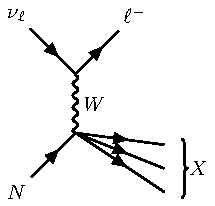
\includegraphics[width=0.4\linewidth]{images/neutrino-nucleon-dis.pdf}
\caption{Диаграмма Фейнмана, соответствующая глубоконеупругому взаимодействию нейтрино с нуклоном через обмен $W$-бозоном. Существует аналогичная диаграмма с обменом $Z$-бозоном, при этом $\ell^- \to \nu$.}
\label{fig:DIS}
\end{figure}

Определим кинематические переменные. Обозначим 4-импульсы: 
$k = (E_\nu, \bm{k})$ — нейтрино, 
$k' = (E_\ell, \bm{k}')$ — лептона в конечном состоянии, 
$p = (M, \bm{0})$ — нуклона в лабораторной системе, 
$p'$ — адронной системы, 
$q = k - k' = p' - p$ — переданный 4-импульс.

Для описания глубоконеупругого рассеяния используется три независимые кинематические переменные: \( Q^2 \equiv -q^2\) и переменные Бьёркена \( x \) и \( y \).
\begin{equation}
  Q^2 \approx 2(E_\nu E_\ell - \bm{k} \cdot \bm{k}') \approx 4E_\nu E_\ell \sin^2\!\frac{\theta}{2},
\end{equation}
где \( \theta \) — угол рассеяния лептона в лабораторной системе. В области глубоконеупругого рассеяния \( Q^2 > 0 \).

Переменные Бьёркена:
\begin{equation}
  x = \frac{Q^2}{2(p \cdot q)}, 
  \qquad 
  y = \frac{p \cdot q}{p \cdot k}.
\end{equation}

Кроме того, полезно использовать:
\begin{enumerate}
  \item \( W^2 = (p + q)^2 = M^2 + 2(p \cdot q) - Q^2 \) — инвариантный квадрат массы адронной системы;
  \item \( s = (k + p)^2 \) — квадрат полной энергии в системе центра масс нейтрино-нуклон.
\end{enumerate}

\subsection{Дифференциальное сечение}

Сечение нейтрино–нуклонного глубоконеупругого рассеяния можно записать в универсальной форме:
\begin{equation}
  \frac{d^2 \sigma_{\text{DIS}}}{dx\,dy} =
  \frac{G_F^2 M E_\nu}{\pi \bigl(1 + Q^2/M_W^2\bigr)^2}
  \sum_{i=1}^{5} A_i(x, y, E_\nu)\, F_i(x, Q^2),
  \label{eq:xsec_general}
\end{equation}
где \( G_F \) — константа Ферми, \( M \) — масса нуклона, \( E_\nu \) — энергия нейтрино, \( Q^2 \) — квадрат переданного импульса, \( F_i(x, Q^2) \) — структурные функции, а \( A_i(x, y, E_\nu) \) — известные кинематические коэффициенты, зависящие от энергии и переменных Бьёркена \( x \) и \( y \).

Структурные функции \( F_i(x, Q^2) \) выражаются через партонные распределения и содержат информацию о внутренней структуре нуклона. Конкретная форма коэффициентов \( A_i \) зависит от свойств начальных частиц, включая их поляризацию. Некоторые подробности приведены в приложении~\ref{app:structure_functions}.

На рис.~\ref{fig:xsec_2d} представлены дважды дифференциальные сечения $\frac{d^2\sigma}{dx\,dy}$ для взаимодействия мюонного нейтрино с протоном через обмен бозоном $W$, рассчитанные при различных энергиях нейтрино и фиксированных значениях переменной $y$. Характерной особенностью этих графиков является то, что с ростом энергии основная часть сечения смещается в область всё меньших значений переменной Бьёркена $x$. Это отражает фундаментальную особенность глубоко-неупругого рассеяния: при больших $Q^2$ всё больший вклад в сечение начинают вносить морские кварки и антикварки. Вклад малых бъёркеновских $x$ в полное сечение обсуждается в разделе~\ref{sec:dis_reliability}.

\begin{figure}[!h]
\centering
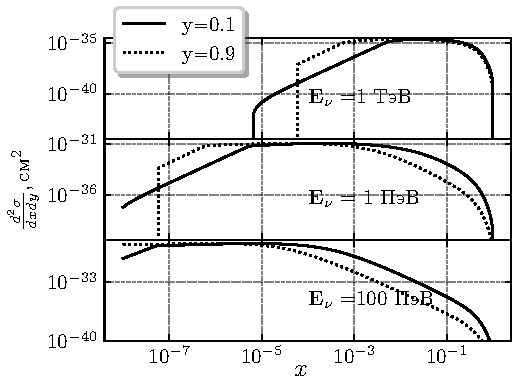
\includegraphics[width=0.8\linewidth]{images/NuProp/xs_vs_xCT10nlo_cc_14_proton.pdf}
\caption{Дважды дифференциальные сечения для рассеяния мюонного нейтрино на протоне за счёт заряженного тока в зависимости от переменной Бьёркена $x$ при различных энергиях нейтрино и фиксированных значениях переменной $y$.}
\label{fig:xsec_2d}
\end{figure}

